%%
%  ******************************************************************************
%  * #file    Szablon_raportu_EN_Latex.tex
%  * #author  Adrian Wójcik   adrian.wojcik(at)put.poznan.pl
%  *          
%  * #commit  Patryk Kościk   koscikpatryk(at)gmail.com
%  *          Modified the template for Projekt przejsciowy purposes          
%  *          
%  * #version 1.0
%  * #date    09-Mar-2022
%  * #brief   PROJPRZEJ
%  *
%  ******************************************************************************
%%  
\documentclass[11pt, a4paper]{article}

\usepackage{SM_template}

% Wypełnijcie te dyrektywy zgodnie z waszym tematem
% \lab      -> NAZWA CZUJNIKA, np.: 'DHT22'
% \comment  -> Króciutki opis co to, np.: 'Cyfrowy budżetowy czujnik temperatury'
%

\lab{Moduł GY-906}
\comment{Cyfrowy czujnik temperatury na podczerwień}
\author{Dawid Wasung}
\addbibresource{bib/GY-906.bib}

% Absolutny zakaz dotykania tego tutaj bo jak dotkiecie to coś jebnie
\university{Politechnika Poznańska}
\faculty{Wydział Automatyki, Robotyki i Elektrotechniki}
\institute{Instytut Robotyki i Inteligencji Maszynowej}
\department{Zakład Sterowania i Elektroniki Przemysłowej}

\nocite{*}


%%
%
% Początek dokumentu
%
%%
\begin{document}

%% Strona tytułowa %%
\mainpage{{GY-906/modul1}}
\newpage

\section*{Opis elementu} \addcontentsline{toc}{section}{Wstęp}
Sercem modułu jest czujnik MLX90614ESF-BAA-000-TU-ND, mierzący temperaturę na podstawie wydzielanego przez obiekt promieniowania cieplnego, które jest emitowane w zakresie podczerwieni - tzw. pirometr. Promieniowanie podczerwone jest niewidzialne dla ludzkiego oka ze względu na długość fal, która zawiera się w przedziale od 780$ nm$ do 1$ mm$, dlatego zadaniem czujnika jest przeanalizowanie promieniowania i na jego podstawie wyznaczenie temperatury badanego obiektu (temperatury powierzchni). Ważną cechą, która jednocześnie może być postrzegana jako wada, jest FOV - stały kąt widzenia. Pole pomiarowe jest zależne od odległości czujnika od obiektu, stąd by osiągnąć jak najdokładniejszy wynik, należy dostosować odległość do wielkości obiektu. Dodatkowo, z pomiarem bezprzewodowym wiąże się pojęcie emisyjności, czyli zdolność danego ciała do emisji promieniowania cieplnego. Jest to wielkość z przedziału od 0 do 1, którą należy predefiniować w programie w zależności od rodzaju materiału, na który skierowany jest czujnik. Tabele emisyjności IR są bezproblemowo dostępne w internecie.
\vspace{0.5cm}
\begin{figure}[h!]
\centering
\begin{subfigure}{.5\textwidth}
  \centering
  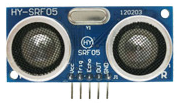
\includegraphics[width=.44\linewidth]{fig/GY-906/zdj_modułu/fig2.png}
  \caption{Pirometr \cite{ArduinoModules:grab}}
  \label{fig:sub1}
\end{subfigure}%
\begin{subfigure}{.5\textwidth}
  \centering
  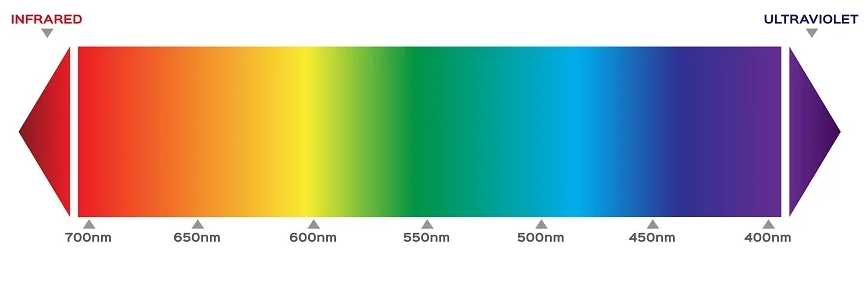
\includegraphics[width=1\linewidth]{fig/GY-906/zasada_dzialania/spektrum.png}
  \caption{Widmo światła \cite{bot:wykres}}
  \label{fig:sub2}
\end{subfigure}
\caption{Wygląd czujnika oraz pogląd na widmo światła}
\label{fig:test}
\end{figure}
\newline
Moduł GY-906 składa się z dwóch rezystorów, dwóch kondensatorów, regulatora napięcia, czujnika MLX90614ESF-BAA-000-TU-ND i czterech wyprowadzeń w postaci pinów męskich. Komunikacja jest możliwa po magistrali I$^{2}$C (SMBus, TWI) oraz za pomocą sygnału PWM. Pracuje z napięciem od 3.3V do 5V. Zakres pomiarowy wynosi od -70$^{\circ}$C do 380$^{\circ}$C, z dokładnością 0.5$^{\circ}$C w zakresie od 0$^{\circ}$C do 50$^{\circ}$C. Rozdzielczość wynosi 0.02$^{\circ}$C dla interfejsu I$^{2}$C, a 0.14$^{\circ}$C dla interfejsu PWM.
\vspace{0.5cm}
\begin{figure}[h!]
    \centering
    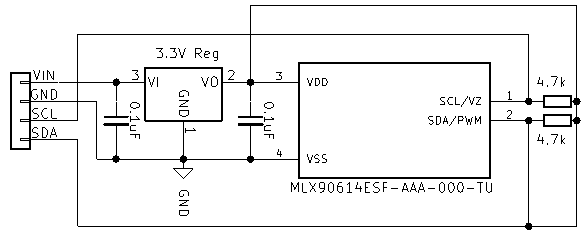
\includegraphics[width=0.8\textwidth]{fig/GY-906/zasada_dzialania/schematt.png}
    \caption{Schemat modułu}
    \label{fig:my_label}
\end{figure}

\newpage
\section*{Użycie czujnika}
Kluczowym elementem prawidłowego funkcjonowania czujnika jest emisyjność, która standardowo znajduje się w pamięci EEPROM (domyślnie ustawiona na 1) i można ją w zależności od potrzeb dowolnie zmieniać. Należy wziąć pod uwagę, że czujnik zwraca informację podaną w stopniach Kelwina i należy ją przeliczyć na stopnie Celsjusza poprzez odjęcie wartości 273.15. Szczegółowe informacje dotyczące zmiany rejestrów czujnika należy sprawdzić w dokumentacji technicznej.
\vspace{0.5cm}
\begin{figure}[h!]
    \centering
    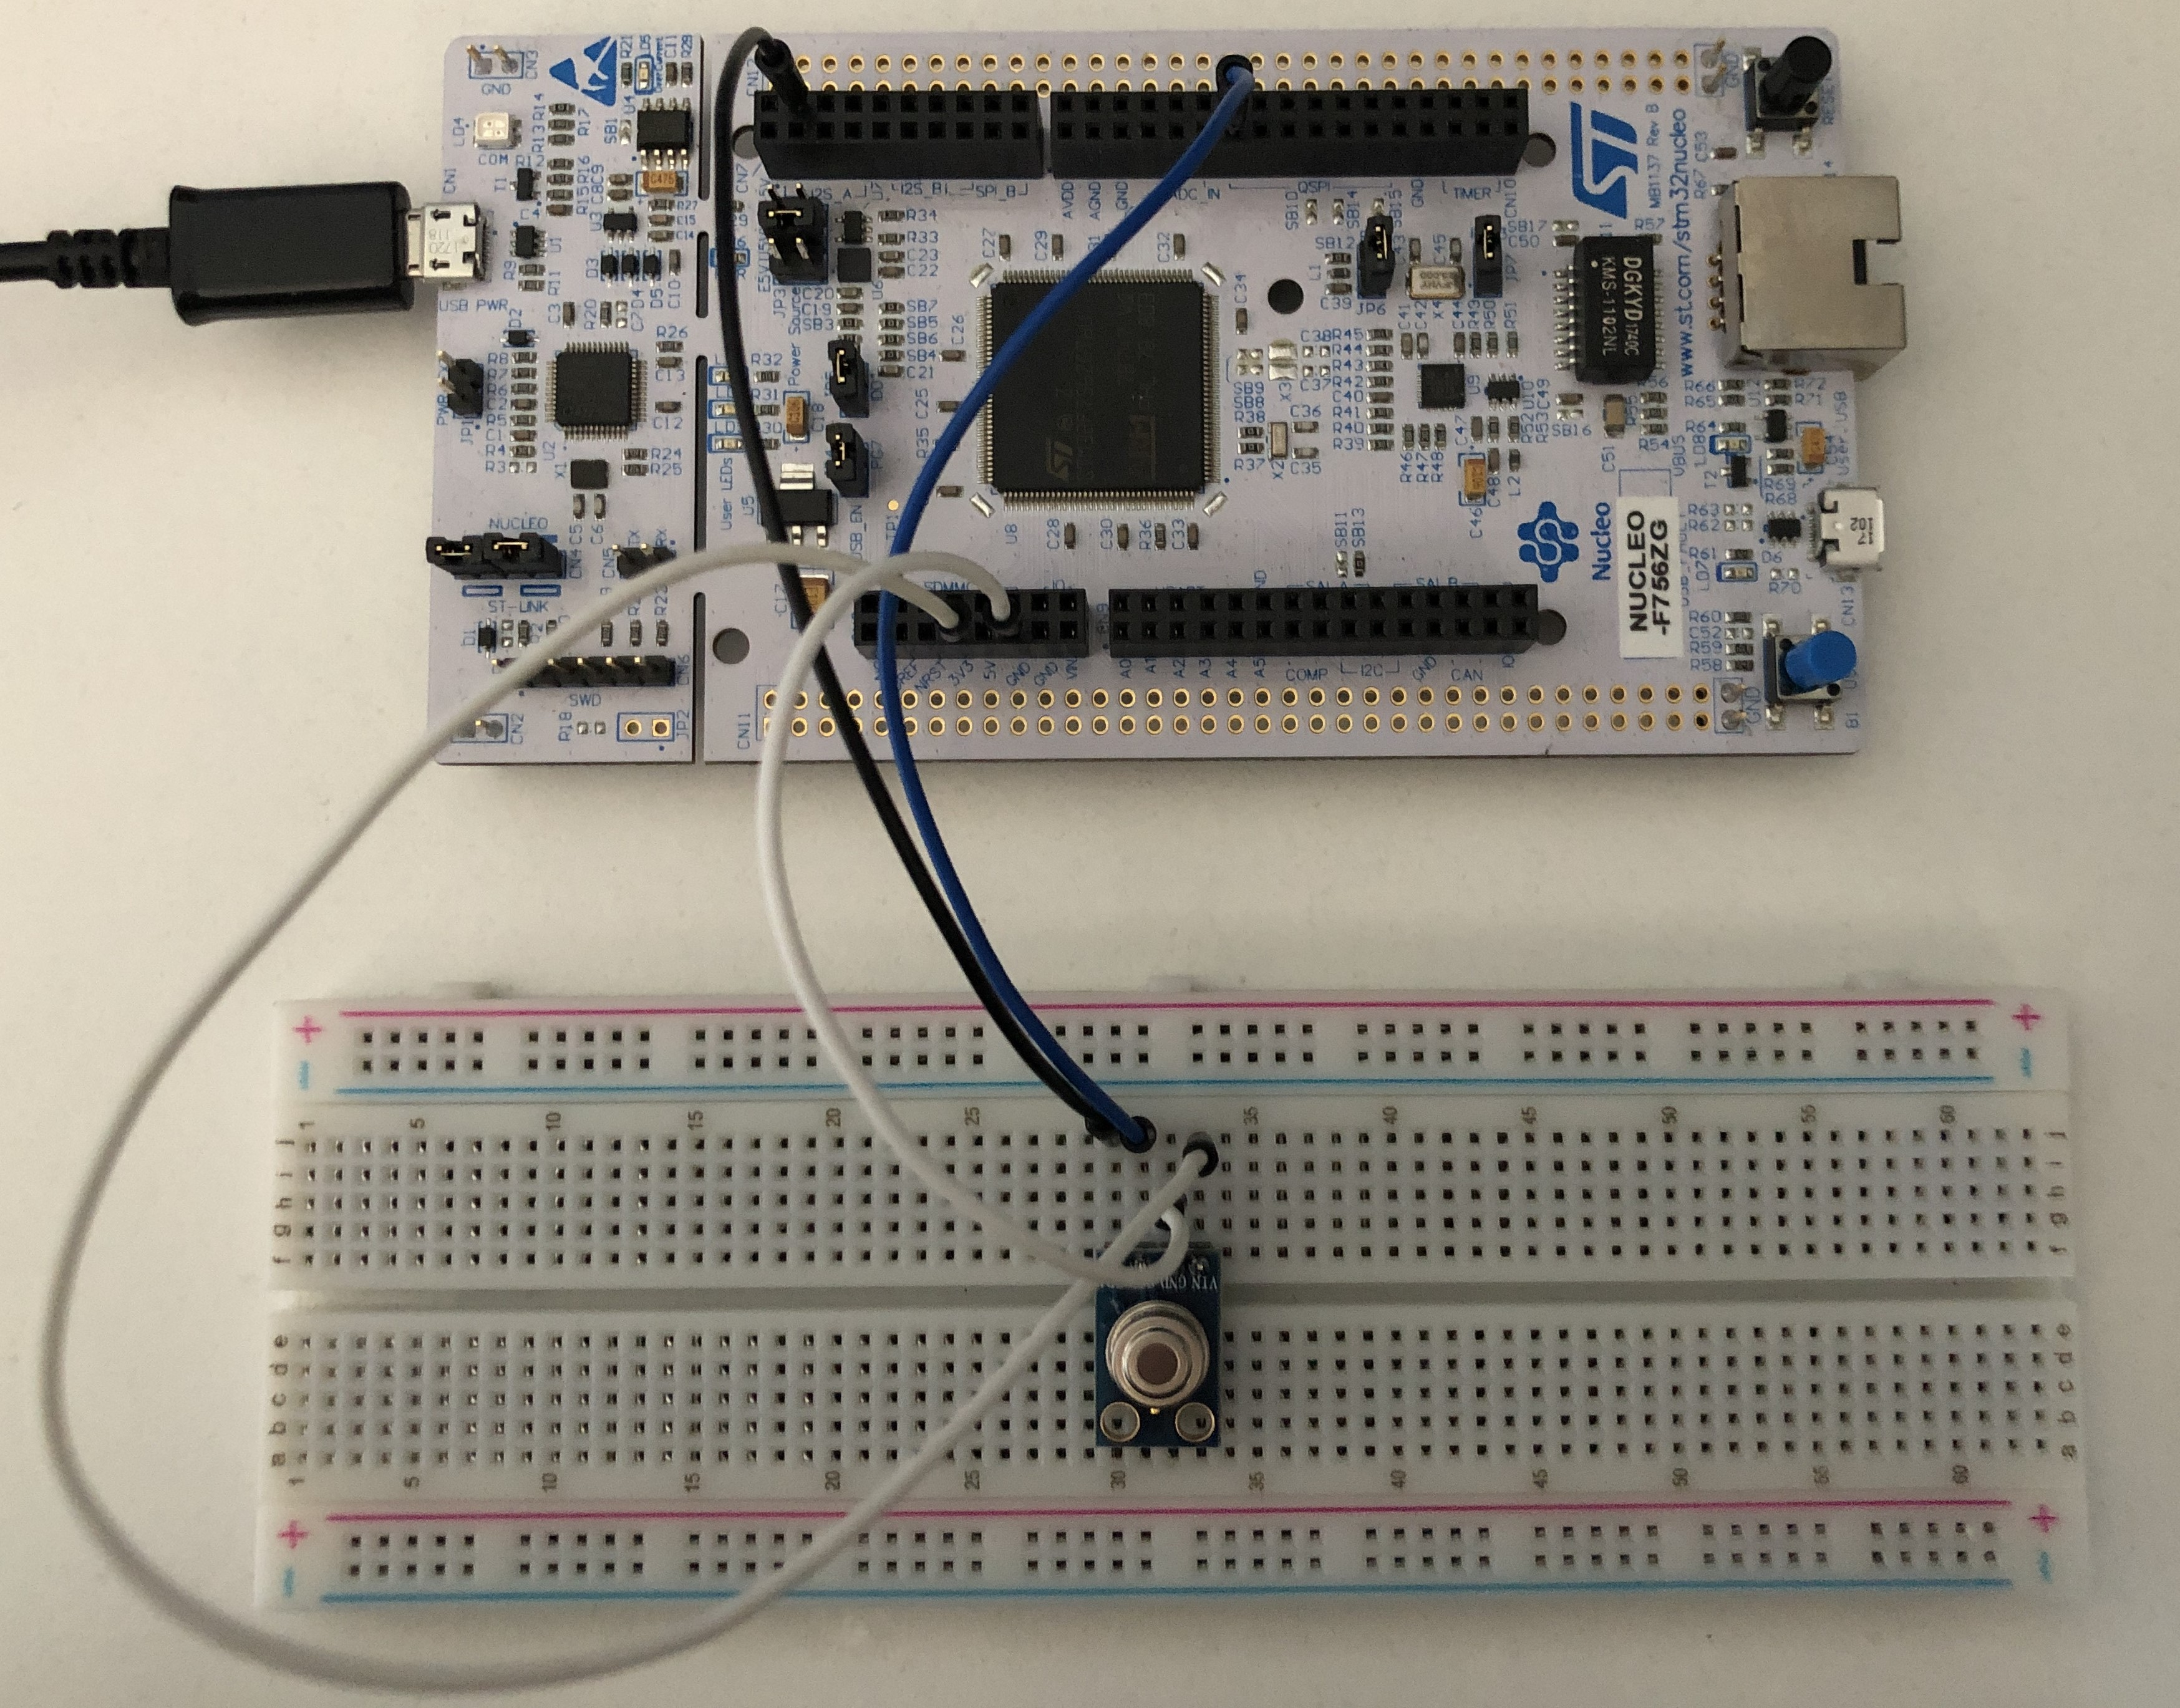
\includegraphics[width=0.6\textwidth]{fig/GY-906/polaczenie_modulu/podlaczenie.jpg}
    \caption{Podłączenie modułu}
    \label{fig:my_label}
\end{figure}
\vspace{0.5cm}
\newline
Jak zostało wspomniane, czujnik można obsłużyć na dwa sposoby (I$^{2}$C z wykorzystaniem SMBus lub PWM). W tym opracowaniu posłużono się pierwszą wymienioną magistralą, warto więc wspomnieć o samym SMBus - jest to niejako pochodna I$^{2}$C. Zasadniczą różnicą będzie PEC (Packet Error Checking), który służy do sprawdzania poprawności przesyłanych informacji; w tym przypadku jedynie podczas zapisu do pamięci EEPROM. W najprostszych słowach, mamy do czynienia z sumą kontrolną CRC-8, która wyliczana jest mając na względzie adres urządzenia, adres rejestru, do którego następuje wpisywanie oraz samej wpisywanej wartości. Rozwiązanie to można obsłużyć na dwa sposoby - podczas kongifuracji mikrokontolera wybrać obsługę SMBus, co upraszcza sprawę i nie trzeba się martwić sprawdzaniem pakietów, lub standardowo wybrać obsługę po I$^{2}$C, ale uwzględnić w przesyłanych danych CRC.
\vspace{0.5cm}
\begin{figure}[h!]
    \centering
    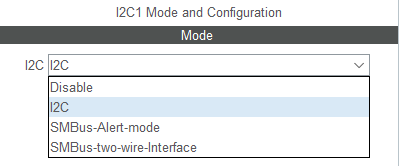
\includegraphics[width=0.6\textwidth]{fig/GY-906/działanie_ukladu/i2c.png}
    \caption{Wybór magistrali}
    \label{fig:my_label}
\end{figure}
\vspace{0.5cm}
\newpage
Emisyjność w programie przykładowym została zdefiniowana na 0.985, co odpowiada wartości emisji cieplnej ludzkiej skóry. Wyniki przedstawiają temperaturę otoczenia oraz mierzonego obiektu.
\vspace{0.5cm}
\begin{figure}[h!]
\begin{subfigure}{.5\textwidth}
  \centering
  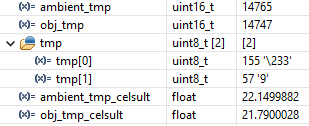
\includegraphics[width=1\linewidth]{fig/GY-906/działanie_ukladu/wynik.png}
  \caption{Temperatura otoczenia oraz mierzonego obiektu }
  \label{fig:sub1}
\end{subfigure}%
\begin{subfigure}{.5\textwidth}
  \centering
  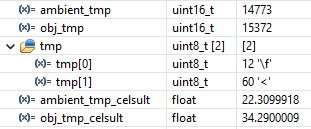
\includegraphics[width=1\linewidth]{fig/GY-906/działanie_ukladu/wynik2.png}
  \caption{Temperatura otoczenia oraz mierzonego obiektu}
  \label{fig:sub2}
\end{subfigure}
\caption{Odczyty poszczególnych wartości}
\label{fig:test}
\end{figure}
\newline
Na powyższych zrzutach zaprezentowane są poszczególne informacje wysyłane przez czujnik - końcowa wartość po przeliczeniu na stopnie Celsjusza jest ukazana przez zmienne ambient\_tmp\_celsult (temperatura otoczenia) oraz obj\_tmp\_celsult (temperatura objektu). W przypadku (a) czujnik nie jest skierowany na obiekt, stąd obie wartości są podobne, natomiast w przypadku (b) do sensora został przyłożony palec; odczytana wartość to temperatura powierzchni skóry.
\vspace{1cm}
\newline
Kod programujący czujnik, wykorzystany do opracowania instrukcji, znajduje się w materiałach dodatkowych zawartych pod koniec rozdziału.
\newline
Film prezentujący działanie układu znajduje się w suplemencie wideo.
\printbibliography[heading=bibintoc]

\end{document}